\documentclass[11pt]{report}
\usepackage{inputenc}
\usepackage{graphicx}
\usepackage{hyperref}
\usepackage{setspace}
\usepackage{lineno}
\usepackage{caption}
\usepackage{subcaption}
\usepackage{wasysym}
\usepackage{latexsym}
\usepackage{amsfonts}
\usepackage{amssymb} 
\usepackage{wrapfig}
\usepackage{lipsum}
\usepackage{changepage}
\usepackage{pgf,tikz,pgfpages}
\usepackage[margin=1.0in,left=1.3in]{geometry}

\begin{document}
\pagenumbering{roman}
\hypersetup{colorlinks=true,linkcolor=black,urlcolor=black}


\begin{titlepage}
\thispagestyle{empty}
\vspace*{0.7cm}
{\centering     
\large
{\Large\bf Assessment of Autism Spectrum Disorder in Toddlers using Speech Features }\\
}
\begin{center}

\bf{Thesis submitted in partial fulfillment of the requirement for M.Tech. Degree}\\
\vspace{0.25cm}
\vspace{0.1cm}
\vspace{1cm}
\it
\vspace{.5cm}
\rm
{\bfseries {Harshit Kumar Gupta}}\\
{\bfseries {Entry No.: 2013EET2369}}\\
{\bfseries {M.Tech.(Computer Technology)}}\\
\vspace{1cm}

{\bfseries {Project Supervisor}}\\
\vspace{0.25cm}
{\bfseries Dr. Santanu Chaudhury}\\
Electrical Engineering Department IIT Delhi\\
\vspace{0.25cm}
{\bfseries Dr. Nandini Chatterjee Singh}\\
National Brain Research Center Manesar\\
\vspace{3cm}
 
\includegraphics[scale=1,keepaspectratio=true]{./images/IITD.png}
 % IITD.png: 282x282 pixel, 72dpi, 9.95x9.95 cm, bb=0 0 282 282
\vspace{1cm}

{\bfseries Department of Electrical Engineering} \\ 
\vspace{0.5cm}
{\bf \LARGE Indian Institute of Technology Delhi}\\ 
\end{center}
\begin{center}
 May 2015
\end{center}
\pagebreak 
\end{titlepage}




\setstretch{1.3}
\setlength{\parindent}{4em}


\begin{center}
\textbf{CERTIFICATE}\\[.5cm]
 \end{center}


This is to certify that the M.Tech. Thesis titled ``Assessment of Autism Spectrum Disorder in Toddlers using Speech Features'' being submitted by Harshit Kumar Gupta, Entry Number 2013EET2369, is a bona-fide work of him under my supervision. The matter submitted has not been replicated anywhere else for the fulfillment of any other objective.

\vspace*{5cm}

\noindent
\textbf{Dr. Santanu Chaudhury}
{\hspace{9cm}May 2015}\\
\textbf{Department of Electrical Engineering}\\
\textbf{Indian Institute of Technology Delhi}\\
Email: santanuc@ee.iitd.ernet.in.\\


\vspace{2cm}
\noindent
\textbf{Dr. Nandini Chatterjee Singh}\\
\textbf{National Brain Research Centre Manesar}\\
Email: nandini@nbrc.ac.in.


\newpage
\begin{center}
\textbf{ACKNOWLEDGMENT}\\
 \end{center}


\medskip 

First of all, I would like to express my sincere gratitude towards Dr. Santanu Chaudhury for giving me an opportunity to work under him and guiding me at every juncture. His wide knowledge and logical way of thinking has been a great value for me. It is for his foresight, altruism and experience only that I was able to complete my major project in time.\\

I would also like to thank Dr. Nandini Chatterjee Singh of National Brain Research Centre Manesar for his valuable inputs regarding Autism Spectrum Disorder. During  visits to NBRC Manesar,Gurgaon, she shared her knowledge about the behavior of Autistic Children which helped me a lot.\\

I would also like to thank National Brain Research Center at Manesar and UW Autism Center, University of Washington, Seattle for providing speech samples of Autistic and Typical Children for this project.



\begin{verbatim}
 

\end{verbatim}
\textbf{Harshit Kumar Gupta}\\
\textbf{2013EET2369}
\newpage


\tableofcontents
\listoffigures
\newpage
\begin{center}
\Large\bf{List of Abbreviations}\\
 \end{center}
\begin{verbatim}
 

\end{verbatim}
\begin{description}
 \item[ASD] Autism Spectrum Disorder
 \item[TD] Typical Development
 \item[FT] Fourier Transform
 \item[FFT] Fast Fourier Transform
 \item[FWT] Fast Wavelet Transform
 \item[STFT] Short Time Fourier Transform
 \item[DWT] Discrete Wavelet Transform
 \item[DWPA] Discrete Wavelet Packet Analysis
 \item[SVM] Support Vector Machine
 \item[HMM] Hidden Markov Model
 \item[CNN] Convolutional Neural Networks 
\end{description}

\newpage
\pagenumbering{arabic}
\chapter{Introduction}
\section{Problem Definition}
The purpose of this project is to recognise the Autism Spectrum Disorder among the children by utilizing the features extracted from their speech.The features helps to detect the neurological disease in its early stage
 The basic idea behind this project was to use speech features to diagnose this neurological disease. For this diagnosis, extraction of features from speech is currently an emerging field. One such neurological disease is Autism Spectrum Disorder in which children lack  communication and interaction ability with society. These children exhibit repetitions in their activity, behavior and functioning. Children with ASD have following characteristics: delayed patterns of speech, missing or abnormal communication gestures, speech patterns diverging from normal, different speech qualities and reduced verbal communication \cite{motor}.\\

It is very important to understand the behavior of autistic children by acoustically monitoring them. It is an open problem in signal processing and machine learning to reliably identify autistic children by speech sample collected in the acoustic environment. Some of the major challenges include simultaneously vocalizing multiple voices and background noise.\\

\section{Motivation}
Currently to diagnose a child with ASD, he/she has to be taken to the Autism Centre to be checked by the doctor. Sometimes diagnosis takes too much time or due to the ignorant nature of parents, it becomes too late to help children to recover from autism spectrum disorder. This project addresses the issue to assess ASD in children using their speech so that children can easily recover in the early stage of ASD.\\  
A technological solution was thus proposed by Dr. Santanu Chaudhury and Dr. Nandini Chatterjee Singh  which could identify the characteristics in speech samples for the classification of autistic children and typical children. If we could identify articulatory signature \cite{arti} in its early stage among children, then treatment of those autistic children can be done at early age so that they can become normal children. We want ASD to be detected easily without the intervention of doctors. So our final objective is to make an android application using which parents can record the speech of their children and upload speech to cloud to know whether their children have symptoms of ASD.



\section{Outline of work done}
The work done can be categorized as per the following objectives:
\begin{enumerate}


\item \textbf{A Review of the State of the Art}
\begin{enumerate}
\item Study of Modulation Spectrum of Speech
\item Study of Pitch Pattens in Children
\item Study of Speech Motor function in Children
\end{enumerate}

\item \textbf{Data}
\begin{enumerate}
\item Data Preprocessing
\item Noise Reduction
\item Framing and Blocking
\item Windowing
\end{enumerate}

\item \textbf{Extraction of  Features from Speech}
\begin{enumerate}
\item Fourier Transform
\item Gabor Transform
\item Discrete Wavelet Transform
\item Discrete Wavelet Packet Analysis
\end{enumerate}

\item \textbf{Overview of Classification Algorithms}
\begin{enumerate}
\item Support Vector Machine
\item Random Forest
\item Hidden Markov Model
\item Convolutional Neural Network
\end{enumerate}

\item \textbf{Classification Models}
\begin{enumerate}
\item MFCC features with SVM and Random Forest
\item Wavelet features with SVM and Random Forest
\item Hidden Markov Model
\item Convolutional Neural Network
\end{enumerate}

\item \textbf{Analysis of Results}
\begin{enumerate}
\item Summary of Classification Accuracy
\item Complexity of Models
\item Conclusion from Results
\end{enumerate}

\item \textbf{Conclusion}
\begin{enumerate}
\item Summary of Work done
\item Contributions Made
\item Future Work
\end{enumerate}

\end{enumerate}
\chapter{A Review of State of Art}
\section{Introduction}
Presently the diagnosis of autism is done using the symptoms  by medical professionals. An autistic child has symptoms such as lack of eye to eye contact, lack of social behavior, stuttering, repetition of activities, uncoordinated actions, aberrant sound production, odd vocal quality, etc. These symptoms start appearing generally in the 3 to 5 year child. Research has shown the brain activity of an autistic child is compromised. However rigid results are not present and the classification is not clear for a mildly autistic patients. \\

Some study has been done on the interaction of autistic children with their parents and also with other children of the same age group. It has been shown that the speech recorded have three different energy bands in the spectro-temporal modulation \cite{arti} with different energies in them, but they are too mixed to be classified on those features. These studies show that when we perform 2D Fourier transform then we get a plot in spectral modulation and temporal modulation. Which shows 3 bands in energy variation for autistic, typical and slow learner children. But those features is not sufficient for classification because there is too much variation in those feature. \\

There are also some researches based on the number of vocalization \cite{motor}. The idea is to capture the stuttering symptoms in autistic children as their words per second count is distinguishably slower than a normal child. While this research is trying to find out the classification of autistic and normal children, no machine learning technique for classification is done till date to forewarn about the possibility of autism in a child.\\

There are many research which has shown that MFCC or wavelet features has given outstanding results  for classification of audio or speech recognition, therefore those feature may also be very useful for our project. Hidden Markov Model with different types of STFT features (Peaks,MFCC etc.) are also useful for modeling non-independent events, so this can be used for modeling syllable frequency. Very recent research focuses on use of deep learning networks for classification of audio  and speech, such as convolutional neural networks, Deep belief networks, Recurrent Neural Network with HMM. These deep networks require large data sets and large computation resources such as use of the GPU(Graphical Processing Units). This is a very emerging field, so we have to explore each method for our problem to find out the best solution.

\section{Study of Modulation Spectrum of Speech}
In this research they analyzed natural sound ensemble by calculating the probability of amplitude envelope of sound. They obtain a Modulation Spectrum \cite{acoustic} by calculating 2-D Fourier transform of the auto-correlation matrix of sound stimulus in its spectrogram. It was shown that sounds cannot have a sudden change in spectral and temporal modulation simultaneously. Speech signals are generally low passed signal and contains most of their spectral modulation power in low temporal modulation.

First Spectrogram (time-frequency representation) is calculated from speech by applying Fourier transform on each frame of signal. Then spectrogram is decomposed as a weighted sum of sine or cos grating of varying period, amplitude and phase. Each grating of spectrogram corresponds to particular sound  called ripple sound \cite{acoustic}. These ripple sounds are sinusoidal function in time and frequency which can be represented as follows:
\begin{equation}
S_i(t,f)=A_i \cos(2\pi\omega_{t,i}t + 2\pi \omega_{f,i} +\phi_i)
\end{equation} 
Spectrogram of sound can be written as sum of ripple components as follows:
\begin{equation}
S(t,f)=A_0 +\sum\limits_i S_i(t,f)
\end{equation}
$A_i$ denote the relative amplitude of modulation depth ($A_0$).Here $\omega_f$ denote temporal modulation frequency in Hertz ,  $\omega_f$ denote spectral modulation frequency and $\phi$ represents initial phase of ripple. Number of frequency units spanned over one second is calculated by $\frac{\omega_t}{\omega_f}$. This term is also known as ripple velocity. Power density of each ripple component is estimated  and plotted in 2-dimensional graph.


An alternate way to calculate the modulation spectrum is to decompose a signal into frequency bands using Gaussian filters. This decomposition results into narrow-band signals. Then an auto-correlation matrix is calculated by cross-correlation of narrow-band signal with all other narrow-band signals including itself. Then all cross-correlation function is averaged over same band to calculate auto-correlation matrix. Then the 2-D Fourier transform of this auto-correlation matrix is plotted which is known as modulation spectrum.

\section{Study of Pitch Patterns in Children}
This study focuses on finding patterns in pitch of children with ASD. In autistic children speech features are found in unusual prosody \cite{melody}. Prosody means only the style of speaking. Prosody can be measured with the help of following measures:
\begin{enumerate}
\item \textbf{Pitch (F0) Measures :} Measure average, max and min pitch.
\item \textbf{Pitch Range :} Variation between max and min pitch.
\item \textbf{Pitch Excursion :} Non native speaker of any language uses pitch of the accented syllable, while native speaker use pitch, frequency and amplitude. If we analyze the pitch contour, then it has more than 13 semitones/Sec. We calculate pitch excursion by following a formula: 
\begin{equation}
Pitch Excursion= \frac{39.863 \log{\frac{F_{max}}{F_{min}}}}{duration}
\end{equation} 
\end{enumerate}

If we see the fundamental frequency contour of each speech chunks, then there is a lot variation in F0 frequency over time. During analysis they found that there is a large gap between the values of Mean Pitch, Mean Pitch Range and Mean Pitch Excursion in different group of children (ASD, DD and TD). This study shows that pitch patterns of children in age 4 to 10 years with ASD are different from normal children of the same age group.



\section{Study of Speech Motor Function in Children}
There have been studies which suggest that we can predict ASD in children with the help of some signature other than their communication and interaction ability. Analysis of speech shows us difference in verbal abilities of children with ASD even at a very early stage. Development of speech motor function \cite{motor} tries to use articulatory features. A measure of articulatory feature is based on acoustic differences in vocalizations. Vocal pattern belongs to two classes of articulatory features which include slow varying or fast varying amplitude.


Spectral analysis techniques are used on speech samples of children to make judgment whether articulatory features are good speech motor function. Two techniques were used for speech sampling, one in which child and one of parent interact and second in which a group of children participate in an activity. A novel technique called \textbf{Speech Modulation Spectrum} was developed to analyze articulatory features. At a particular time if we analyze variation in energy on a range of frequency, then that is called spectral modulations. Similarly at a particular frequency if we analyze variation in energy on a range of time then that is called temporal modulations.


Speech Modulation Spectrum is generated by taking the 2-D Fourier transform of the spectrogram. This modulation spectrum contains bands of three different types of information. These articulatory features \cite{arti} are as follows.
\begin{enumerate}
\item \textbf{Syllabic Rhythm (SR) :} Region between 2 to 10 Hertz. 
\item \textbf{Formant Transition (FT) :} Region between 25 to 40 Hertz.
\item \textbf{Place of Articulation (POA) :} Region between 50 to 100 Hertz.
\end{enumerate} 


Modulation Spectrum is a plot of Temporal modulation v's Spectral modulation in which it shows the power distribution with respect to SR, FT and POA. The area inside contour of these regions defines articulatory features. At last correlation between articulatory features and behavioral features is analyzed to find patterns.




\section{Conclusion}
The idea being worked upon here is to forecast the onset of autism in children by using the voice of children. An extensive database is being created though mobile and Internet applications to gather a large amount of data. This data is being used to train the classifier for predicting the beginning of autism based on various features that will be explained in the following chapters in detail. In the next chapter, we will learn about data-set and feature extraction techniques established in signal processing and machine learning approach for classifying them.


\newpage
\chapter{Data}
\section{Introduction}
In this chapter, we will describe the dataset. After that we will explain how to pre-process speech samples and how to remove noise from samples. For feature extraction we need to divide the whole signal into frames, so the procedure for framing will be explained. Before applying any transform we need to prevent spectral leakage from the end and start of frame, so we apply window operation on frames.

\section{Description of Dataset} 
 We performed the experiment on dataset provided from National Brain Research Centre, Manesar, Gurgaon which was originally obtained from the University of Washington, Seattle. At the UW Autism Center, these speech samples were collected from ADOS (Autism Diagnostic Observation Schedule) and PCI (Parent Child Interaction).The  Dataset contains 40 speech samples,20 speech samples from autistic and typical children each. All audio files were 16-bit digitized and sampled at a rate of 44.1 KHz. These samples are used to extract articulatory features.

\section{Noise Reduction}
Speech samples were collected in very noisy environment so we listen to samples using Audacity, a free audio processing software and remove background noise. Then we apply wavelet based de-noising method to remove remaining noise.
Then we amplify speech samples and also perform normalization on audio. Audio normalization is performed to gain in amplitude of speech by stretching audio from average or peak amplitude to a target level.


\section{Framing And Blocking}
In framing we divide continuous 1 D signals into small frames of N samples, then we take next frame by shifting M samples, this causes adjacent samples to overlap by M-N samples.Choice of M and N is an application specific maintaining constraint M $<$ N. We choose frame size sufficiently small to capture significant information.\\
\begin{equation}
TotalFrames= \frac{(S-M)}{(N-M)}
\end{equation}
Where S is the total number of samples and N is the number of samples in the frame and M is the number of samples shift for next frame.\\
If we have 40 ms frame length, then it carries pitch modulations information, i.e it offers high frequency resolution and if we take 5 ms frame length, then it carries information about change in timbre i.e. it offers high time resolution. So the selection of these parameters is very pivotal when the process uses the feature extraction techniques  like MFCC, STFT, DWT etc.  \\

\section{Windowing}
To minimize spectral leakage at the start and end of frame it is necessary to apply windowing to frame.In this process we multiply window function and frame together. Window function is also called tapering function.
There exists many window function. Some are listed below.
\begin{enumerate}
\item Rectangular Window
\item Triangular Window
\item \textbf{Hanning Window}
\begin{equation}
W_(n)=0.5(1-  \cos(\frac{2\pi n}{N-1}))
\end{equation}
\item \textbf{Hamming Window} It optimizes maximum side lobe of signal.
\begin{equation}
W_(n)=\alpha -\beta \cos(\frac{2\pi n}{N-1})
\end{equation}
where $\alpha =0.54$ and $\beta =1- \alpha=0.46$
\begin{figure}[h]
\centering
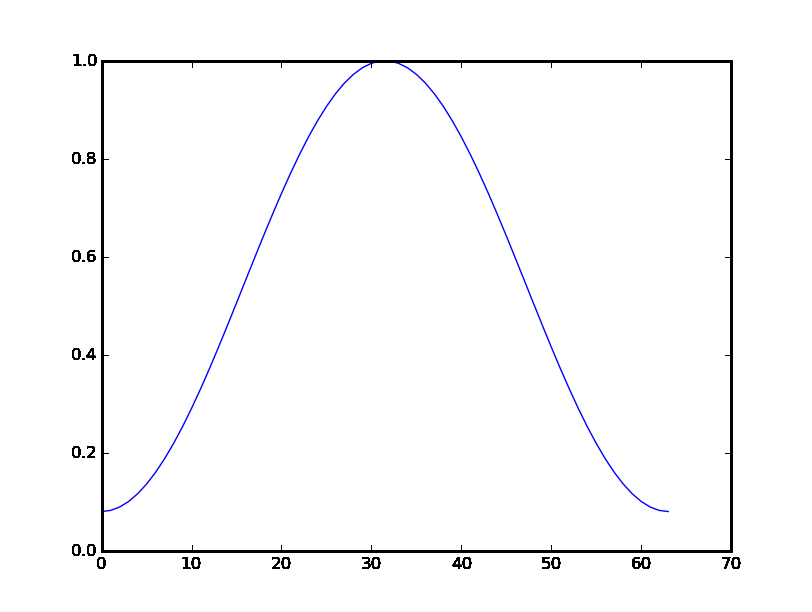
\includegraphics[scale=.50]{./images/hamm.png}
\caption{Hamming Window}

\end{figure}
\end{enumerate} 

\section{Conclusion}  We have explained above how to pre-process audio and the intuition behind framing and blocking. We also understood window function.The choice of window function influences the result drastically. Windowing operation on frame is necessary before applying any signal processing technique for feature extraction. Next chapter deals with feature extraction from signal frame by frame. 
\newpage
\chapter{Description of Feature Extraction Techniques} 
\section{Introduction}
In this chapter we shall discuss which signal processing techniques will be used for feature extraction tasks. The choice of the parameters and feature extraction methods varies with applications.Same method may give the good result on particular data set while for other it may fail.   So choice of parameters in these techniques are purely experimental. I chose to use Fourier transform because it gives us frequency component of the signal and it is the basic building block of many other techniques. Short Time Fourier transform was used because it removes disadvantages of FT and applies FFT on small frames to get frequency resolution of frames. After that if we apply some additional steps, then we obtain MFFC coefficients or peaks in each frame signal. We also chose wavelet transform because it offers us multi-resolution analysis without compromising  the loss of the information  of the signal compared to previous techniques. In subsequent sections these techniques are described in detail with their working, advantages and disadvantages.

\section{Fourier Transform}
Fourier Transform is used for conversion of one signal (function) from one basis to another like convert time domain speech signal to frequency domain signal which helps us to find contribution of each different frequency components. Sine and Cosine represent basis function in $L^2$ space. So we can express any periodic function in terms of sine and cosine. 

\textbf{Analysis formula} for Discrete Fourier transform can be written as follows:
\begin{equation}
X_{k}=\sum\limits_{n=0}^{N-1} x_{n} e^ {-j\frac{2\pi}{N}nk} 
\end{equation}
We evaluate above formula for k=0,1,... upto N-1 when we convert time domain signal to frequency domain.

According to \textbf{Parseval's Theorem}, if we change the underlying basis, the energy of the signal will not change.
\begin{equation}
\sum\limits_{n=0}^{N-1} {|x_{n}|}^2 =\frac{1}{N}\sum\limits_{k=0}^{N-1} {|X_{k}|}^2
\end{equation}

We can also get original signal back using \textbf{Synthesis formula} or \textbf{Inverse Fourier Transform} which can be written as follows for k=0,1,... upto N-1:
\begin{equation}
x_{k}=\frac{1}{N}\sum\limits_{n=0}^{N-1} x_{n} e^ {-j\frac{2\pi}{N}nk} 
\end{equation}

Calculation of Fourier Transform has $O(N^2)$ complexity  which has very high computational cost when we have long signal. So one faster algorithm is used for this transform which is known as \textbf{Fast Fourier Transform(FFT)}.FFT has $O(N\log_{2}N)$ cost for calculation of N point signal.Points given by FFT are symmetrical, so only $\frac{N}{2}+1$ points are unique and sufficient to represent FFT. Therefore we keep only first $\frac{N}{2}+1$ points and discard the rest.








\section{Mel Frequency Cepstral Coefficient}
These coefficients are mainly used in speech recognition, music information recognition and genre classification. 
MFCC also represent the state of the human auditory system.
Mel Frequency Cepstrum (MFC) is a power spectrum representation of signal at each window which is linear cosine transforming of a log power spectrum on a nonlinear Mel scale of frequency. Group of MFC coefficient is known as Mel-Frequency Cepstral Coefficients (MFCC).MFCC can be calculated using Yaafe \cite{yaafe} feature extraction library.



\begin{figure}[h]
\centering
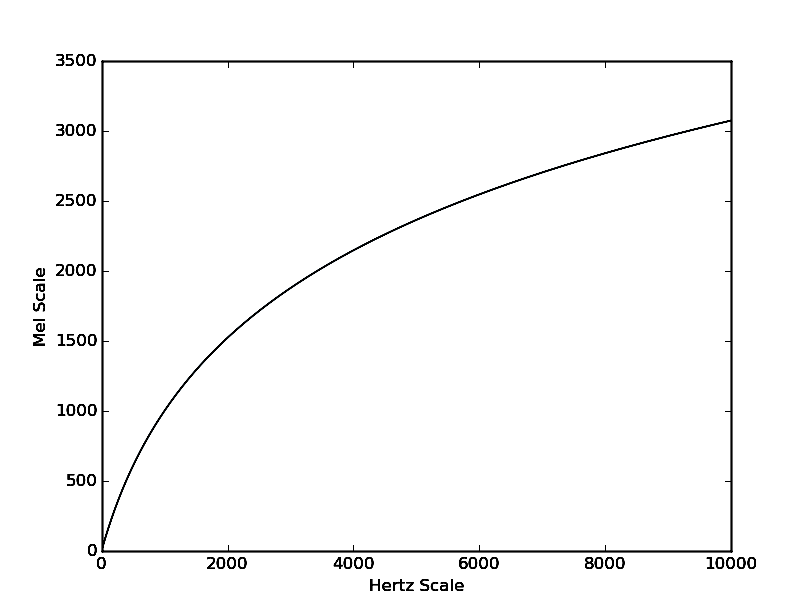
\includegraphics[scale=.4]{./images/mel.png}
\caption{Hertz Scale vs Mel Scale}

\end{figure}
The formula  to convert from frequency to Mel scale is:
\begin{equation}
M_{f}=1125 \ln(1+\frac{f}{700}) 
\end{equation}
Following is a detailed procedure of calculation of MFCC:

\begin{enumerate}
\item Divide the signal in the short windowed frame.
\item Calculate periodogram estimate of the power spectrum for each frame.
\item Map power spectrum on Mel frequency scale.
\item Take log of all Mel power bands.
\item Take DCT of Mel log power spectrum. 
\item Keep only some first DCT coefficients, discard the rest.
\end{enumerate}
\begin{figure}[h]
\centering
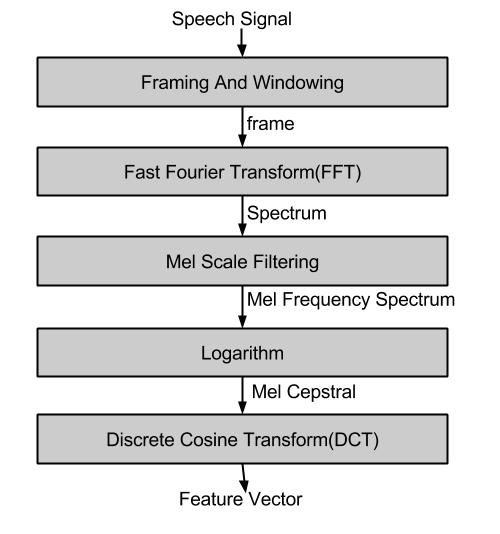
\includegraphics[scale=.6]{./images/mfcc.png}
\caption{MFCC Feature Extraction}

\end{figure}


\subsection{Discrete Cosine Transform (DCT)}
DCT calculates real part of the Fourier transform.First DCT coefficient is called the DC coefficient, which is the lowest frequency in block. If we are given a list of N values in a vector Q then their DCT coefficients can be given by:
\begin{equation}
F(u)=\sqrt{\frac{2}{N}} C(u) \sum\limits_{x=0}^{N-1} \cos(\frac{(2x+1)u\pi}{2n})Q(x)
\end{equation}
for u=0,1,.....N-1


$C(u) = \frac{1}{ \sqrt2 } $ if u==0 otherwise
$C(u) =0 $  







\newpage
\section{Gabor Transform}
When we analyze the signal in frequency domain then information in time domain is lost. We can't know which frequency component occurs, at which time. As \textbf{Heisenberg's Uncertainty Principle} suggests that we can't have good resolution both in time and frequency domain. Gabor transform allows us to have frequency resolution within a time window. If we use skinny time window for analysis, then we capture high frequencies with time localization, but if we use fat window, then we capture low frequencies which are not localized in time.
So we take a time window like hanning or hamming and find the Fourier transform of the signal only in that window. Gabor transform is also known as \textbf{Short Time Fourier Transform}.We can use scipy \cite{scipy} for signal processing tasks.

 

\begin{figure}[h]
\centering
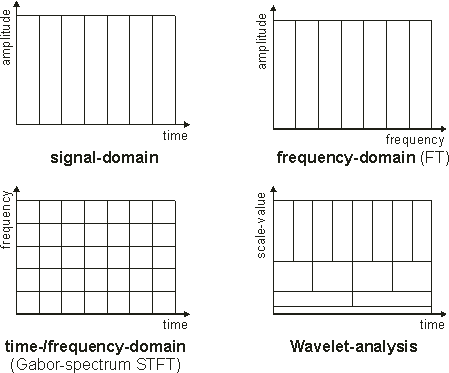
\includegraphics[scale=.6]{./images/domain.png}
\caption{Signal resolution at different domains}
\end{figure}

\subsection{Spectrogram}
Spectrogram offers us visualization of spectral components w.r.t. time. It is actually a time vs frequency representation of signal but this does not have accurate resolution instead we use time window to calculate STFT of signal. We plot frequencies in each time window. In this plot color depth of each point indicate number of times that frequency occurs in that time window \cite{acoustic}. 

\begin{figure}[h]
\centering
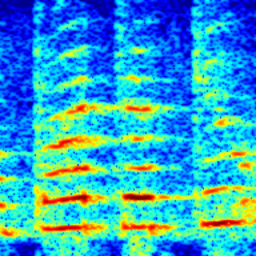
\includegraphics[scale=.7]{./images/spec_asd.png}
\caption{Spectrogram of autistic child}
\end{figure}

\begin{figure}[h]
\centering
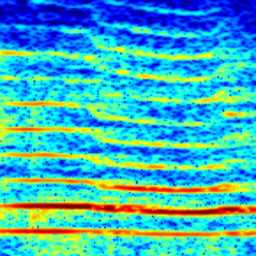
\includegraphics[scale=.7]{./images/spec_td.png}
\caption{Spectrogram of typical child}
\end{figure}


\newpage
\section{Wavelet Transform}
Wavelet are functions which provide an orthonormal basis for function in $L^2$ space like sine and cosine are an orthonormal basis in the Fourier transform. Wavelet provides us multi-resolution analysis.



All wavelets are derived from mother wavelet, so wavelet with scale s and time $\tau$ is equal to mother wavelet normalized by the square root of scale s and shifted in time by $\tau$ and change in scale s.
\begin{equation}
\psi_{s,\tau}(t)=\frac{1}{\sqrt{s}}\psi(\frac{t-\tau}{s})
\end{equation}
where s represents scale and $\tau$ represents time.

Formula of \textbf{wavelet transform} can be written as follows:
\begin{equation}
\gamma(s,\tau)=\int f(t)\psi_{s,\tau}^*(t)dt
\end{equation}
where $\psi_{s,\tau}^*$ represent complex conjugate of mother wavelet.

Formula of \textbf{inverse wavelet transform} can be written as follows:
\begin{equation}
f(t)=\int \int \gamma (s,\tau)\psi_{s,\tau}(t)d \tau ds
\end{equation}


\subsection{Properties of Wavelets}
Wavelet basis function has following properties:
\begin{enumerate}
\item Orthogonal (basis functions are perpendicular to each other)
\item Each vector is normal vector 
\item Output of the transform will have the same energy as input.
\item Sparsity (so many coefficients are zero) 
\item Linear Time Complexity for transformation.
\end{enumerate}

\subsection{Wavelet Families}
Wavelets are organized into groups called Wavelet Family. Most commonly used families are:
\begin{enumerate}
\item \textbf{Haar }: These are used for extracting image feature for object recognition and real-time face detector.\begin{figure}[h]
\centering
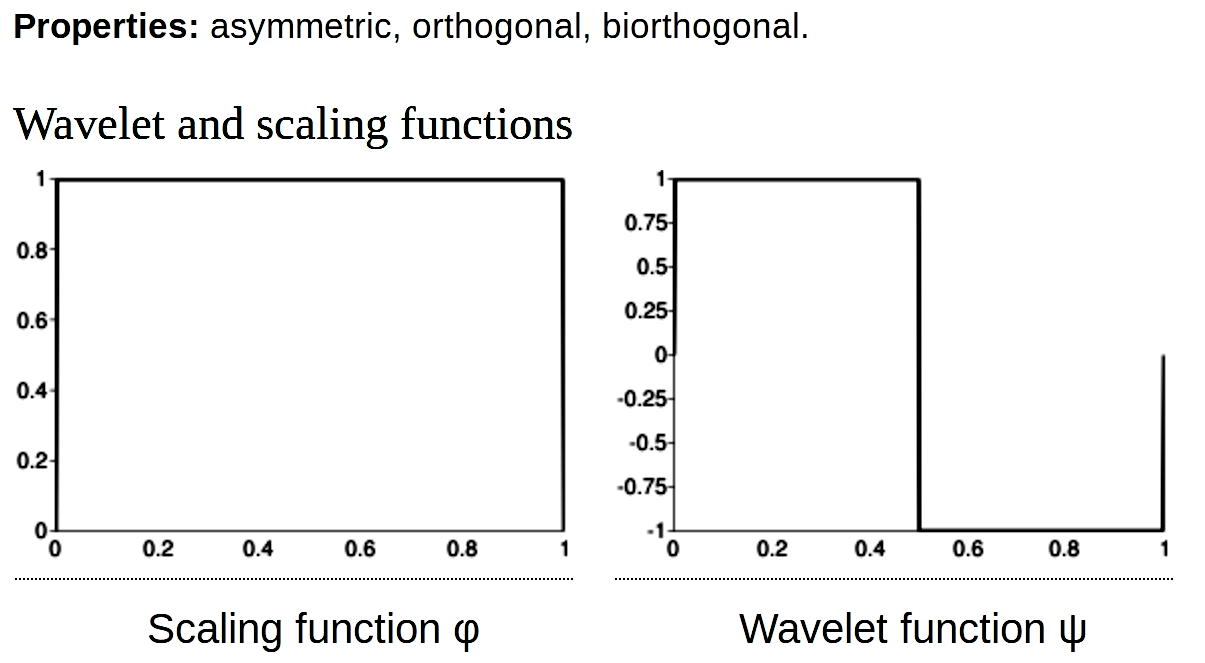
\includegraphics[scale=.25]{./images/haar.png}
\caption{Haar  Wavelet}
\end{figure}
\item \textbf{Daubechies }: These are used for image or speech denoising and feature extraction for speech classification. \begin{figure}[h]
\centering
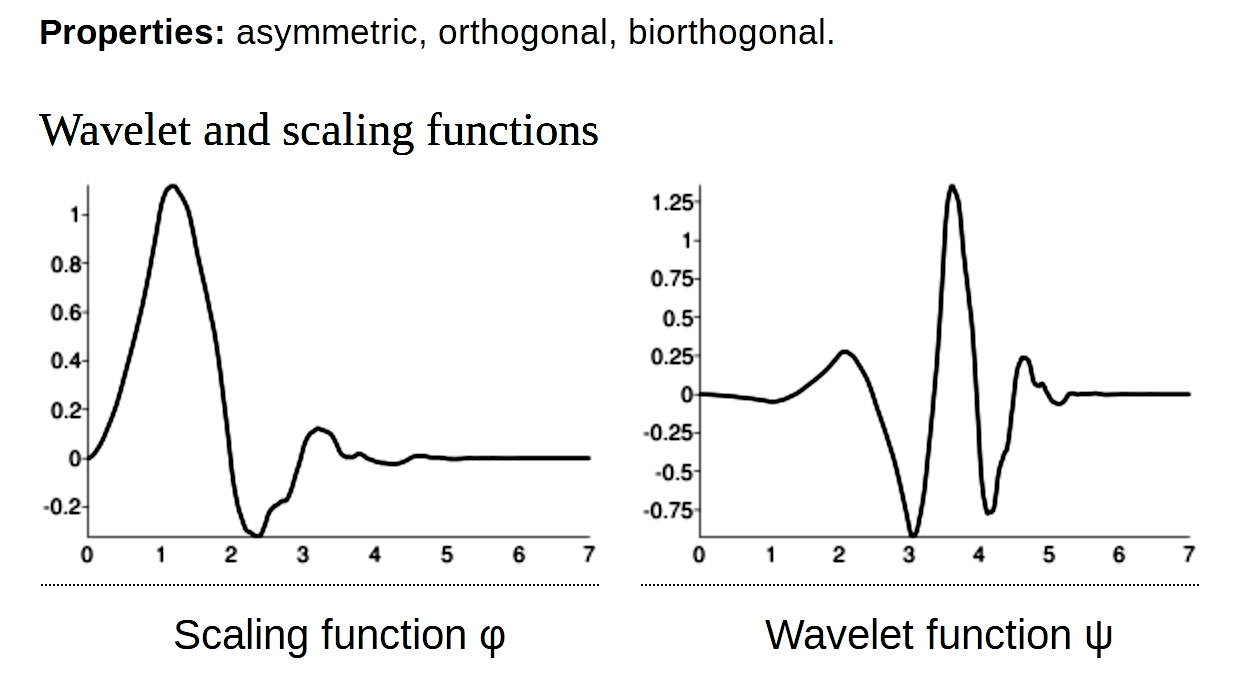
\includegraphics[scale=.3]{./images/db4.png}
\caption{Daubechies 4 Wavelet}
\end{figure}

\item Symlets
\item Coiflets
\item Biorthogonal




\item Reverse Biorthogonal
\item "Discrete" Meyer
\end{enumerate}



\subsection{Types of Wavelet Coefficient}
After wavelet Transform we find two types of coefficients:
\begin{enumerate}
\item \textbf{Approximation Coefficients} : These coefficients represent high scale, low frequency component of the signal. We calculate these coefficients by applying low decomposition filter (LDF) on the signal and then applying down-sampling by a factor of 2.
\item \textbf{Detail Coefficients} : These coefficients represent low scale, high frequency component of the signal. We calculate these coefficients by applying high decomposition filter (HDF) on the signal and then applying down-sampling by a factor of 2.
\begin{figure}[h]
\centering
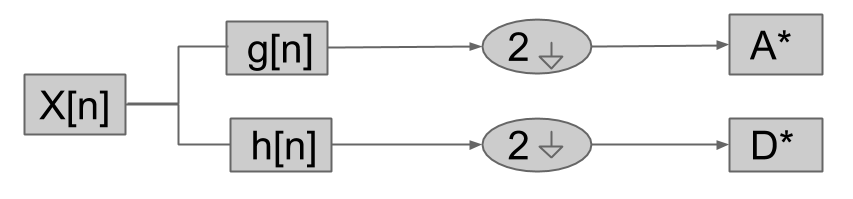
\includegraphics[scale=.5]{./images/dwtcoeff.png}
\caption{Decomposition filer on signal}
\end{figure}
\subsection{Significance of Wavelet Coefficients}
Wavelet transform allows us exceptional localization in both time domain via translation of mother wavelet and in scale (frequency) domain via dilation. Translation and dilation operations are applied to mother wavelet to calculate wavelet coefficient, which represent similarity (co-relation) between wavelet and a localized section of signal. So wavelet transform better resolves high frequency component in temporal resolution and low frequency component in scale resolution.




\subsection{Scalogram}
Scalogram is a time vs scale representation of the signal. For this we do cross-correlation of chosen wavelet and our signal and then plot results. This is scale-1. Next we dilate wavelet (stretch it by some factor) then again, do cross-correlation of this new waveform with our signal then we get scale-2 plot. So scalogram \cite{sca} shows the result of performing a cross-correlation of signal with wavelet at different scales (dilation and stretch factor).
In this plot bright spot means we get a good cross-correlation score between stretched wavelet and signal. Bright spots indicate where the peaks and the valleys of stretched and shifted wavelet align best with the peaks and the valley of signal. Dark means no alignment, dimmer means some peaks and valleys align up, but brightest where all peaks and valley align.  
\begin{figure}[h]
\centering
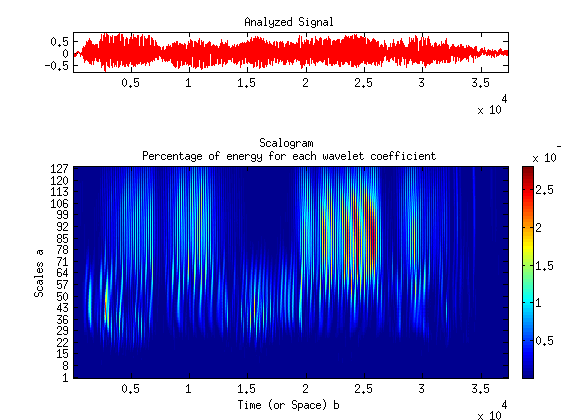
\includegraphics[scale=.6]{./images/sca_asd.png}
\caption{Scalogram of autistic child}
\end{figure}

\begin{figure}[h]
\centering
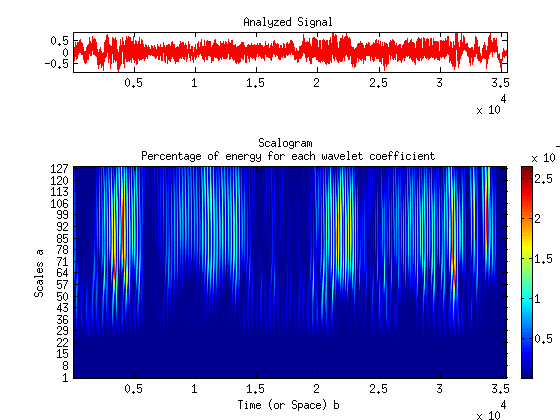
\includegraphics[scale=.6]{./images/sca_td.png}
\caption{Scalogram of typical child}
\end{figure}

\newpage
\subsection{Discrete Wavelet Transform}
Discrete Wavelet Transform utilizes low frequency component (approximation coefficient). In this transform we iteratively perform low pass filtering and high pass filtering at each level on approximation coefficient only.
This multiple level decomposition is also called Wavelet decomposition tree.
\end{enumerate}\begin{figure}[h]
\centering
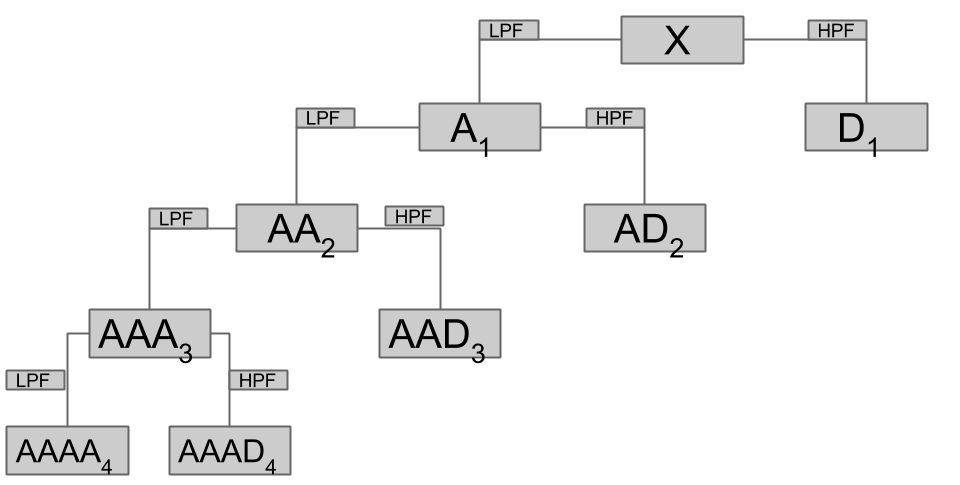
\includegraphics[scale=.45]{./images/dwt.png}
\caption{Discrete Wavelet Transform}
\end{figure}








\newpage
\subsection{Discrete Wavelet Packet Analysis}
Discrete Wavelet Packet Analysis utilizes both low frequency component (approximation coefficient) and high frequency component (detail coefficient). In this transform we iteratively perform low pass filtering and high pass filtering at each level.

\begin{figure}[h]
\centering
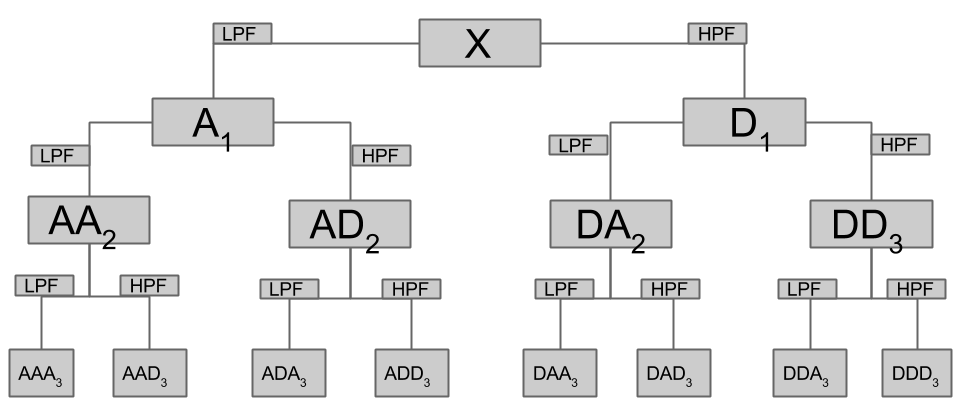
\includegraphics[scale=.5]{./images/dwpa.png}
\caption{Discrete Wavelet Packet Analysis}
\end{figure}

\section{Conclusion}
This chapter describes working, advantages and disadvantages of feature extraction techniques used in this projects. If we use FFT then it takes $O(N\log_{2}N)$ time for calculation of N point Fourier Transform. When we use Short time Fourier Transform, then we apply linear time windowing operation  w.r.t. to size of frame followed by FFT to each frame so it take $O(F*N\log_{2}N)$ time where F is the total number of frames and there are N points in the frame. Wavelet transform takes $O(N)$ time for calculation in one frame. So when we calculate it for multiple frames this complexity is multiplied by the number of frames. So Fast Wavelet transform (FWT) is faster than Fast Fourier Transform and also captures temporal and spectral content together. In the next chapter, we will explain machine learning classifier which will use these extracted features.



\chapter{Classification Algorithms}
\section{Introduction}
In this chapter I will explain which machine learning techniques will be used for classification tasks. Selection of classifier depends on the number of samples and number of features. I choose to use Support Vector Machine because it works well even with small dataset and Random Forest because it is less prone to over-fit when training on a large number of features .Hidden Markov Model was used as it generate a probabilistic model for non-independent  events which occur at different time .Convolutional Neural Network was used because it will automatically learn features from all the samples which out explicitly defining kernel to extract features and later classify them. We have used $x_{i}$ and $y_{i}$ to represent a feature vector and class label of $i^{th}$ samples. N represents total number of samples. In later section, every algorithms is described in detail with its working, advantages and disadvantages.   

\section{Support Vector Machine (SVM)} 
This classifier constructs a hyperplane or a set of hyperplanes in high or infinite dimensional space. This classifier minimizes empirical classification error and maximize geometric margin. This is also known as a maximum margin classifier. It can also implement non-linear classifiers by applying kernel trick to the maximum margin classifier.
There are two types of SVM classifiers:
\begin{enumerate}
\item C-SVM
\item nu-SVM
\end{enumerate}

\subsection{C-SVM}
In this SVM, we try to minimize the following error function during training.
\begin{equation}
E(w)=\frac{1}{2} w^T w + C \sum\limits_{i=0}^{N} \xi_{i}
\end{equation}
Error function E(w) is subjected to following constraints:
$y_{i}(w^T \phi(x_{i} + b)\leq 1- \xi_{i}$
and $\xi_{i}\leq 0$.

\subsection{nu-SVM}
In this SVM, we try to minimize the following error function during training.
\begin{equation}
E(w)=\frac{1}{2}w^T w - \upsilon \rho + \frac{1}{N}\sum\limits_{i=0}^{N}\xi_{i}
\end{equation}
Error function E(w) is subjected to following constraints:
$y_{i}(w^T \phi(x_{i} + b)\leq \rho-\xi_{i}$
and $\xi_{i}\leq 0$ and $\rho \leq 0$.

\subsection{Advantages of SVM}
Following are main advantages of SVM.
\begin{enumerate}
\item Works well in very high dimensional data.
\item If the number of dimensions is greater than number of samples, then  it still works fine.
\item Only a subset of points contributes in decision making, so it takes very less space on memory and those points are called support vector.
\item Supports a variety of kernel functions.
\end{enumerate}
 
\subsection{Disadvantages of SVM}
Following are main disadvantage of SVM.        
\begin{enumerate}
\item If number of features are greater than the number of samples, then model  is likely to give poor performance.
\item No direct estimation of probability. 
\end{enumerate}
Implementation of SVM can be used from scikit-learn \cite{sklearn}.

\newpage
\section{Random Forest}
Random Forest is an ensemble classifier that consists of many decision trees. The final output class is the mode of set of output classes obtained from the individual output of the various decision trees. Random forest combines the random selection of feature and bagging.\textbf{Bagging (Bootstrap Aggregation) }of decision trees reduces the bias of a single tree. It uses permutation to determine variable importance. We assume all trees are drawn from an identical distribution which minimizes loss function at each node in a given tree.\\

\subsection{Terminology used in Random Forest }
\textbf{Out of Bag (OOB) Error Rate}: There is no need for separate testing or cross validation in random forest. We calculate how many times predicted class from it is not equal to true class from votes of each built tree and when this error is averaged over all cases called OOB error.\\
\textbf{Variable Importance}: Subtract votes-count for correctness in the variable-m-permuted OOB data from votes-count for correct class in the untouched oob data. The importance score for variable m is calculated by averaging the local importance score obtained from each individual decision tree.

\subsection{Algorithm of Random Forest}
Algorithm of random forest can be written as follows:\\
For each tree performs following 1 to 3 tasks-
\begin{enumerate}
\item Fit decision tress minimizing a loss function using 2/3rd of the samples.
\item Predict classes of remaining samples and calculate the mis-classification rate which is equal to out of bag error rate.
\item We permute the variables and calculate the out of bag error. An increase in out of bag error from original indicate the importance of variable.
\item Aggregate OOB error and importance measure from all trees is used to determine the overall OOB error rate and variable importance measure.
\end{enumerate}

\subsection{Advantages of Random Forest}
Advantages of random forest can be written as follows:
\begin{enumerate}
\item Very accurate
\item Efficient for large databases.
\item Handles so many features without feature deletion.
\item Estimation of variable importance in classification. 
\item Reports internal unbiased estimate of the generalization error.
\item Balance between high bias and high variance.
\item Estimate missing data.
\item Accurate even if large amount of data is missing.
\end{enumerate}


\subsection{Disadvantages of Random Forest}
Disadvantages of Random forest can be written as follows:
\begin{enumerate}
\item Over-fit for noisy classification dataset.
\item Biased in  of categorical variable with different number of levels.
\item The Variable importance score for categorical variable is not reliable.

\end{enumerate}
Implementation of Random Forest can be used from sklearn \cite{sklearn}.



\newpage
\section{Hidden Markov Model}
The Hidden Markov model is a generative probabilistic model. In this model sequence of internal hidden state generate a sequence of observations.We can not observe hidden states directly. We assume the transitions between hidden states to be first order Markov Chain.\\

\subsection{Notation of HMM} 
Notations  used for HMM are as follows:
\begin{enumerate}
\item \textbf{N}: number of possible states
\item \textbf{M}: number of possible observations
\item \textbf{X}: \{$q_{1}$,...$q_{N}$\}(finite set of states)
\item \textbf{O}: \{$v_{1}$,...,$v_{M}$\} (finite set of observations)
\item \textbf{$X_{t}$}: random variable denoting the state at time t (state variable)
\item \textbf{$O_{t}$}: random variable denoting the observation at time t (output variable)
\item \textbf{$\sigma$}: {$o_{1}$,...,$o_{T}$} (sequence of actual observations) 
\end{enumerate}

\subsection{Parameters of HMM} 
Parameters for hidden Markov model can be given as follows:
\begin{enumerate}
\item \textbf{transition probabilities $A=[a_{ij}]$}
\begin{equation}
a_{ij} = Pr(X_{t+1} = q_{j} |X_{t} = q_{i}) 
\end{equation}

\item \textbf{observation probabilities $B=[b_{i}]$}
\begin{equation}
b_{i}(k) = Pr(O_{t} = v_{k} | X_{t} = q_{i})
\end{equation}

\item \textbf{initial state distribution ${\pi}=[{\pi}_{i}]$}
\begin{equation}
{\pi}_{i} = Pr(X_{0} = q_{i}) 
\end{equation}
\end{enumerate}

\begin{figure}[h]
\centering
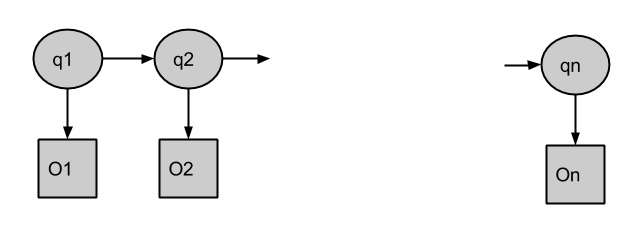
\includegraphics[scale=.5]{./images/hmm.png}
\caption{Hidden Markov Model}
\end{figure}

\subsection{Solution of fundamental problems of HMM}
Following algorithms are used for solution of HMM problems.
\begin{enumerate}
\item \textbf{Forward-Backward algorithm} 
Evaluation problem can be solved using a dynamic programming technique known as Forward-Backward algorithm. This gives us most likely observation sequence.
\begin{equation}
\alpha_T(i)=Pr(O_1=o_1,...,O_T=o_T, X_T = q_i | \lambda)= Pr(\sigma, X_T = q_i | \lambda)
\end{equation}

$\alpha$ values enable us to solve this problem by marginalizing
\begin{equation}
Pr(\sigma | \lambda) = \sum\limits_i^{N} Pr(o_1,...,o_T, X_T = q_i | \lambda) = \sum\limits_i^{N} \alpha_T(i)
\end{equation}

we need $\beta$ values in expectation maximization algorithm which we compute as follows.
\begin{equation}
\beta_t(i) = Pr(O_t+1=o_t+1,...,O_T=o_T | X_t = q_i, \lambda)
\end{equation}
\newpage
\textbf{Steps in Algorithm }
\begin{enumerate}
\item In forward pass we calculate alpha values:
\begin{enumerate}
\item \begin{equation}
\alpha_1(i) = \pi_i * b_i(o_1)
\end{equation}

\item \begin{equation} \alpha_{t+1}(j) = [\sum\limits_i^{N} \alpha_t(i) a_{i,j}] b_j(o_{t+1})
\end{equation}
\end{enumerate}
           
\item In backward pass we compute beta values:
\begin{enumerate}
\item \begin{equation}
\beta_T(i) = 1
\end{equation}
\item \begin{equation}
\beta_t(i) = \sum\limits_i^{N} a_{i,j} b_j(o_t+1) \beta_{t+1}(j)
\end{equation}
\end{enumerate}
\end{enumerate}  

\item \textbf{Viterbi Algorithm}
Decoding problem can be solved using a dynamic programming technique known as Viterbi algorithm. In this  we compute most likely state sequence by stating  observation of length zero and then of length one. After this, we repeat the procedure until we get a state sequence which has the highest probability.

\textbf {Algorithmic Details}
\begin{enumerate}
\item Initialization: For i=1....N
\begin{enumerate}
\item \begin{equation}
delta_1(i) = \pi b_i(o_1)
\end{equation}
\item  \begin{equation}
\Phi_1(i) = 0
\end{equation}          
\end{enumerate}

\item Recursion: For t=2.....T and j=1........N
\begin{enumerate}
\item \begin{equation}
 \delta_t(j) = max_i [\delta_{t-1}(i)a_{i,j}]b_j(o_t)
\end{equation}
\item \begin{equation}
\Phi_t(j) = argmax_i [\delta_{t-1}(i)a_{i,j}]
\end{equation}
\end{enumerate}           

\item Termination:
\begin{enumerate}
\item \begin{equation} p* = max_i [\delta_T(i)]
\end{equation}
\item \begin{equation}
i*_T = argmax_i [\delta_T(i)]
\end{equation}
\end{enumerate} 

\item Reconstruction: For t = T-1,T-2,...,1
 \begin{equation}
  i*_t = \Phi_{t+1}(i*_{t+1}) 
\end{equation}
\end{enumerate}

\item \textbf{Baum-Welch algorithm}
Learning problem can be solved by an iterative Expectation-Maximization (EM) algorithm, known as the Baum-Welch algorithm.
\\
given model and observation sequence, if we are at state $q_i$ at time t the probability of being at state $q_j$ at time t+1 is given by 
\begin{equation}
	\xi_t(i,j) = Pr(X_t = q_i, X_t+1 = q_j | \sigma, \lambda)
\end{equation}
we can compute above probabilities with the help of forward backward variables.
\begin{equation}
\xi_t(i,j) =\frac{\alpha_t(i) a_{i,j} (o_{t+1}) \beta_{t+1}(j)}{Pr(O | \lambda)}
\end{equation}        
given model and observation sequence we compute probability of being at state $q_i$ at time t is given by
\begin{equation}
\gamma_t(i) = Pr(X_t = q_i | \sigma, \lambda)
\end{equation}

By marginalizing gamma we can obtain
\begin{equation}
        \gamma_t(i) = \sum\limits_j \xi_t(i,j)
\end{equation}
expected number of transitions from $q_i$  is given by\begin{equation}
\sum\limits_{t=1}^T \gamma_t(i)
\end{equation} 
expected number of transitions from $q_i$ to $q_j$ is givenn by \begin{equation} \sum\limits_{t=1}^T  \xi_t(i,j)\end{equation}\\


\textbf{ Steps in Algorithm }
\begin{enumerate}
\item Randomly choose initial parameter $\lambda =\{A,B,\pi \}$


\item Reestimate the parameters
\begin{enumerate}

\item \begin{equation}
bar{\pi}_i = \gamma_t(i) 
\end{equation}
\item \begin{equation}                           
bar{a}_{i,j} =\frac{\sum\limits_{t=1}^{T-1}  \xi_t(i,j)}{\sum\limits_{t=1}^{T-1} \gamma_t(i)}                            
\end{equation}
\item \begin{equation}
bar{b}_j(k) = \frac{\sum\limits_{t=1}^{T-1} \gamma_t(j) l_{o_t = k}}{\sum\limits_{t=1}^{T-1} gamma_t(j) }                                  
\end{equation}
\end{enumerate}

    where $l_{o_t = k} = 1$ if $o_t = k$ and 0 otherwise. 
\item Let $bar{A} = {bar{a}_{i,j}}$, $bar{B} = {bar{b}_i(k)}$, and $bar{\pi} = {{bar{\pi}_i}}$.
\item Set $bar{\lambda}$ to be ${bar{A}, bar{B}, bar{\pi}}$.
\item If $\lambda = bar{\lambda}$ then quit, else set $\lambda$ to be $bar{\lambda}$ and return to Step 2. 
\end{enumerate}


\end{enumerate}





                        



\newpage
\section{Convolutional Neural Network}
These are also called as convnet \cite{cnn} . These are supervised deep neural networks. This approach is inspired from working of human visual perspective feeds. There are different types of layers in CNN like convolution, pool, loss, ReLU etc. layers.

\subsection{Convolution }
This is an operation on two function f and g which produce filtered version of f using filter g. Convolution perform smoothing or sharpening. When it is applied to 2-D functions it is used for feature detection, edge finding, image matching, motion detection, etc.
\begin{equation}
f(x) * g(x)= \int_{-\infty}^{\infty} f(\tau) g(x- \tau) d\tau
\end{equation} 
\begin{equation}
f(x,y) * g(x,y)= \int_{-\infty}^{\infty}\int_{-\infty}^{\infty} f(\tau_1,\tau_2) g(x- \tau_1,y-\tau_2) d\tau_1 d\tau2
\end{equation} 

\subsection{Characteristics of CNN}
This approach is currently dominating other deep learning approaches because:
\begin{enumerate}
\item \textbf{Sparse Connectivity}: This allows us to use different copies of the same feature detector with different positions.
\item \textbf{Weight Sharing}: This is also known as \textbf{Feature Maps} which allows us to use several different feature types, each with its own map of replicated weights.
\item \textbf{Sub Sampling}: This is achieved with the help of averaging or max pooling feature maps.
\end{enumerate}

\subsection{Different layers in CNN}
Following is the list of types of layers used in CNN.
\begin{enumerate}
\item \textbf{Convolution Layer }: In this layer features are extracted by applying the convolution operation between input data and kernel.A kernel with same parameter is applied to the overall data over which further operations are done.
\item \textbf{Dropout  Layer}: This layer dropout same features which we obtained from the same regions of data, thus reducing the risk of over-fitting. Each node in the neural network is dropped with a certain probability and the result is observed. The result is classified as either a spike in the output or just an insignificant change and based on the result the node is dropped. It also makes the training a lot faster.
\item \textbf{ReLU Layer}: Any deep neural network without non-linear operation at some hidden layer will perform similar to Logistic Regression. To introduce non-linearity we have to use functions like sigmoid, tanh, or RelU. RelU is the most popular in deep neural networks because it is more similar to the biological neuron.  
\item \textbf{Loss layer}: This layer is used to compute the error in the network so that errors can be back-propagated to tune parameters of the network.
\end{enumerate}

\subsection{Advantages of CNN}
\begin{enumerate}
\item \textbf{Equivalent activities}: Replicated features do not make the neural activities invariant to translation. They make activities to be equivalent.

\item \textbf{Invariant knowledge}: During training if some feature is useful at some position, then during testing also feature at that position will be useful.
\end{enumerate}

\section{Conclusion}
This chapter describes working ,advantages and disadvantages of classifiers used in this project. A later chapter will describe combinations of feature extraction techniques with these classifier which helps in understanding the intuition behind the working and performance model used. 

\newpage 
\chapter{Models used for classification}
\section{Introduction}
In this chapter I will explain models proposed for classification. Here we will compare all models with each other their working, performance and at last we will compare the complexity of each model. Complexity of the model depends on the size of the data set because that determine the complexity of optimization function to be minimized. We have used probabilistic(HMM), non-probabilistic(SVM), ensemble based method (Random Forest), deep neural network(CNN) where each classifier belongs to a different type of category. Here we have explained each model deal with what parameters to be optimized and we  will analyze diverse nature of these models.
\section{Classification using SVM and Random Forest with MFCC}
\subsection{Feature Construction from MFCC coefficients}
We apply MFCC feature extraction technique speech frames to feature. Then we divide MFCC Feature into histogram bins. We use frequency of each bin as a feature. MFCC features are state of art for classification tasks. Depending on the scenario we have to use feature construction technique from MFCC features.
\begin{figure}[h]
\centering
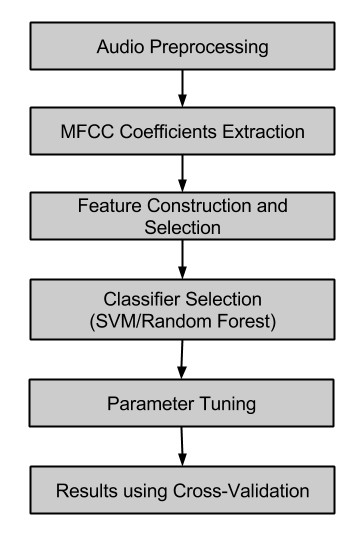
\includegraphics[scale=.6]{./images/mfcc_flow.png}
\caption{Classification with MFCC features}
\end{figure}

\subsection{Selection of Parameters of Classification Model}
\subsection{Support vector Machine}
For a selection of parameters we build different models with different parameters and select the model which gives better results. Following are different parameters which we tuned by exhaustive search.
\begin{enumerate}
\item \textbf{kernel :} linear,polynomial, radial basis function (RBF) kernel
\item \textbf{C :} Penalty Parameter 
\item \textbf{gamma :} Kernel coefficient for poly and RBF kernel
\item \textbf{degree :} Degree of polynomial kernel
\end{enumerate}

\subsection{Random Forest}
For the selection of parameters we build different models with different parameters and select the model which gives better results. Following are different parameters which we tuned by exhaustive search.
\begin{enumerate}
\item \textbf{No of Estimators :} No of trees to be build for classification
\end{enumerate}
 


\section{Classification using SVM and Random Forest with DWT and DWPA} 
\subsection{Feature Construction from DWT or DWPA coefficients}
We apply DWT or DWPA on speech frames to get approximation and detail coefficients on several levels of decomposition. Then we take the sum and the variance of the coefficients of frames at each level. Then we take difference between these sum and variance of successive frames \cite{ad}.

If F is all approximation or detail coefficients after LPF and HPF and i represent frame number then feature is constructed from following:
\begin{enumerate}
\item mean($F_i$)
\item std($F_i$)
\item mean($F_i$) - mean($F_{i-1}$)
\item std($F_i$) - std($F_{i-1}$)
\item mean($F_{i+1}$) - $2*mean$($F_{i}$) + mean($F_{i+1}$)
\item std($F_{i+1}$) - $2*std$($F_{i}$) + std($F_{i+1}$) 
\end{enumerate} 
 
\subsection{Selection of Number of decomposition levels and Mother  wavelet}
We should choose mother wavelet which should be computationally efficient and provide better distinguishing characteristics. We perform experiments from Haar, Symlet, Daubechies wavelet using different levels from 1 to 8. Then the number of decomposition level and mother wavelet is decided by their performance. We experimented a lot to get the best number of level of decomposition and best mother wavelet. We found out Daubechies-8 (db8) with 5 levels of decomposition gives the best results with classifiers.

\subsection{Selection of Parameters of Classification Model}

\begin{figure}[h]
\centering
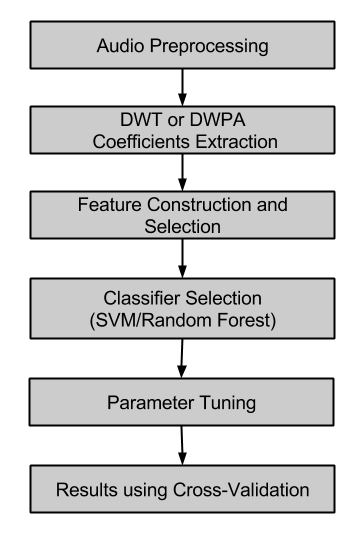
\includegraphics[scale=.6]{./images/dwt_flow.png}
\caption{Classification with DWT/DWPA features}
\end{figure}
\textbf{Support vector Machine}
For the selection of parameters we build different models with different parameters and select the model which gives better results. Following are the different parameters which we tuned by exhaustive search.
\begin{enumerate}
\item \textbf{kernel :} linear,polynomial, radial basis function (RBF) kernel
\item \textbf{C :} Penalty Parameter 
\item \textbf{gamma :} Kernel coefficient for poly and RBF kernel
\item \textbf{degree :} Degree of polynomial kernel
\end{enumerate}

\textbf{Random Forest}
For the selection of parameters we build different models with different parameters and select the model which gives better results. Following are different parameters which we tuned by exhaustive search.
\begin{enumerate}
\item \textbf{No of Estimators :} No of trees to be build for classification
\end{enumerate}

\section{Classification using HMM}
\subsection{Feature Construction using Peaks Detection}
I have extracted features by detecting peaks in frequency for each frame of signal. For feature extraction from speech has moved the current art of state to Deep learning, but still these features works fine with audio. If we use STFT for finding peaks in frequency. For STFT we apply the FFT to each frame, so we have used FFTW \cite{FFTW05} routines which are very fast for calculation of FFT.
\subsection{Algorithm for Peak Detection}
\begin{enumerate}
\item Let X be the length of window on each frame which we use on signal.
\item Divide the window in three parts like left,right and center.
\item Use Max function on each the of 3 parts of a window.
\item If the function value on center is greater than the  function value on left and right parts then goto the next condition otherwise goto 6.
\item We have found the peak if the function value on center is actually in middle position.
\item Move to the next frame and repeat whole process.
\item When we process whole data, then we sort all obtained peaks in decreasing order by their amplitude. 
\item Output only the first six peaks from each frame.
\end{enumerate}


\subsection{Working of HMM model}
\begin{figure}[h]
\centering
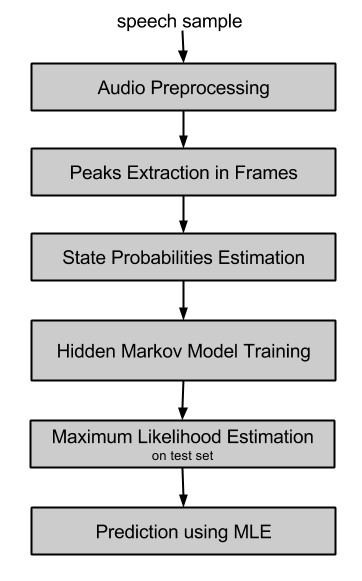
\includegraphics[scale=.6]{./images/hmm_flow.png}
\caption{Classification with HMM Model}
\end{figure}
We will use Maximum Likelihood estimation (MLE) to maximize the probabilities of estimations and learn HMM parameters. In this classification task only Forward, Backward Algorithm and Baum-Welch Algorithm is needed.\\
The required tasks have been accomplished through implementation of various combinations of feature extraction algorithm from signal processing and classification algorithms of  machine learning. We have found peaks in frequency, but we need probabilities to train HMM, so we will normalize the observations. Each frame has a set of peaks. We can obtain state probabilities by dividing each frame peak by the sum of all frame peaks.
These probabilities will show the distribution of peaks. Equal peaks will cause equal probabilities, and unique distribution will lead to a unique set of attributes. \\
HMM learns transition probabilities between frames using state probabilities \cite{hmm} obtained from the peaks. Now we will train 2 separate HMM model one for autistic class and one for typical class. When we need to predict the class, we give features of test samples to both models then  the model which gives higher probabilities for maximum likelihood is the  predicted class. 
 


\section{Classification with CNN}

This network is similar to large multilayer Perceptron (MLP) sparsely connected and tries to model biological neural network of visual system. It uses so many layers of convolution  and pooling together to filter features from data and performs sampling. We repeat combinations of these two layers until we get sufficient object level(high level) features. 
Caffe \cite{jia2014caffe} is open source implementation of CNN which we can define your layers of our model and easily experiment with it.






\subsection{Responsibilities of CNN Layers}
\begin{figure}[h]
\centering

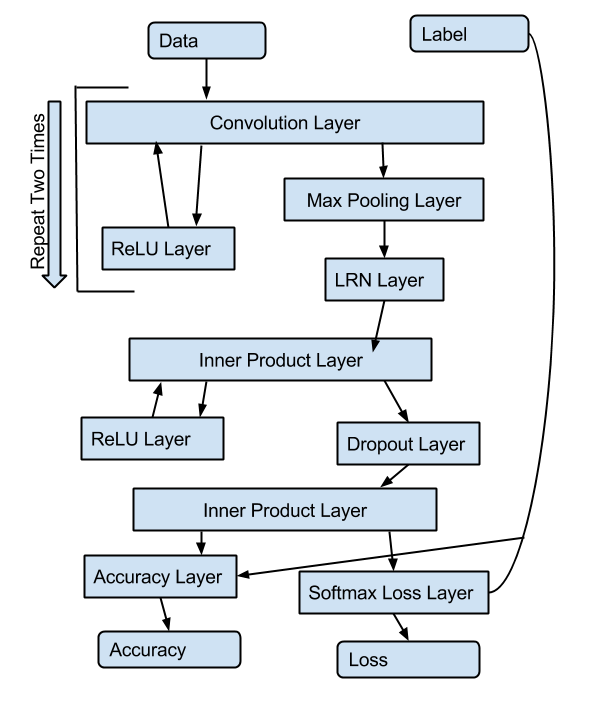
\includegraphics[scale=.7]{./images/cnn.png}

\caption{Classification with CNN}
\end{figure}
We have used the following types of layers in CNN and these layers perform following tasks:
\begin{enumerate}



\item \textbf{Convolutional layer}
In this type of neural network, convolution kernel is  calculated by back-propagation algorithm while previously kernel or filter were fixed like Gaussian blur, sobel, etc. We have so many kernels in each layer and each of them works on entire image with weight sharing. Convolution operation extracts necessary information from the image. The capacity of a neural net varies, depending on the number of layers. Initial layers extract information like edges and line. Next layers combine those low level features into curves, shape like features. At last these layers represent object level features. The first convolution layers will obtain the low-level features, like edges, lines and corners. 



\item \textbf{Pooling layer}
It ensures activity invariance by producing the same result even if the object has some translation. This layer either computes the maximum or the average to reduce variance. When we take maximum then this is also called "Max Pooling Layer".

\item \textbf{Dropout layer}
Fully connected Layers has a large number of parameters which  causes over-fitting. Dropout improves training speed. It is like dropping out neurons, which in turn will not contribute to forward pass and back propagation.

\item \textbf{Local Response Localization}
It normalizes all features in a local input domain. Due to scaling of features network will be generalized.

\item \textbf{Rectified Linear Units(ReLU) layer}
This layer introduces non-linearity into the model without affecting receptive fields of convolution layer otherwise, without these outputs of models with many layers will be just a linear combination of inputs.
There are many activation functions which introduce non-linearity such as:
\begin{enumerate}
\item \textbf{ReLU} $ f(x) =  max(0,x)$
\item \textbf{hyperbolic tangent} $f(x) = |tanh(x)|$
\item \textbf{sigmoid function} $f(x)=\frac{1}{1+e^{-x}}$
\end{enumerate}

\item \textbf{Loss layer}
We have different loss functions for different scenario such as-
\begin{enumerate}
\item \textbf{Soft-max loss :} For predicting single class out of K mutually exclusive classes. 
\item \textbf{Sigmoid cross-entropy loss} For predicting single class out of K independent classes. 
\item \textbf{Euclidean loss} For regression to real-valued labels.
\end{enumerate}
\end{enumerate}



\subsection{Structure of CNN Model}
Following structure was used for classification of spectrogram:
\begin{enumerate}
\item Layer 1: Input layer with data and label.
\item Layer 2a: Convolution layer with 128 kernels of size 5x5 and stride of 1 and in-place ReLU layer is also used.
\item Layer 2b: Pooling layer with kernel size 3 and stride 2.
\item Layer 2c: LRN layer for locally normalizing input to it.
\item Layer 3a: Convolution layer with 96 kernels of size 11x11 and stride of 4 and in-place ReLU layer is also used.
\item Layer 3b: Pooling layer with kernel size 3 and stride 2.
\item Layer 3c: LRN layer for locally normalizing input to it.
\item Layer 4a: Convolution layer with 64 kernels of size 3x3 and stride of 2 and in-place ReLU layer is also  used.
\item Layer 4b: Pooling layer with kernel size 3 and stride 1.
\item Layer 5: Inner Product which is fully connected layer.
\item Layer 5b: RelU unit is used in-place with Inner product.
\item Layer 5c: Dropout Layer is also used in-place with Inner Product to drop redundant feature.
\item Layer 6: Inner Product which is fully connected layer
\item Layer 7a: Accuracy Layer which uses label from input layer to predict accuracy of model.
\item Layer 7b: Loss Layer which calculates error in each unit with help of label so that these error can be back-propagated  in the network.
\end{enumerate}

For training of CNN we have used Mini-Batch Gradient descent as optimization algorithm. In this algorithm error is calculated on a small set of data and that error is back-propagated, then error is calculated on another set of data and the same procedure is repeated. After convergence of CNN we have obtained kernels which will give feature upon convolution with input data. In subsequent layers we convert low level features to high level feature and that is used in a fully connected layer of neurons to get predicted classes.



\section{Conclusion}
Here we have explained all classification methods with their feature extraction techniques.The complexity of each model depends on feature extraction techniques and optimization algorithm used. Wavelet with SVM is outperforming all other techniques, but when we will get more data from sources, then we will be able to train CNN better and we hope that CNN will give better results. Wavelet with SVM is fastest and CNN requires highest computation resources while the other models such as HMM will need less computation time than CNN but more than that of wavelets. There is a large scope of experimentation for different speech feature combination and classification algorithms. Results have been tabulated in a later section.


\newpage
\chapter{Results} 
\section{Introduction}
In this section we will compare the classification accuracy and complexity of all the used models. The results produced by any classification model depend on quality of features and number of samples. As we have 40 samples of speech to cross validate the results of any above model, we cannot strongly suggest that these are best classification results. Accuracy of models may change as we change the size of the dataset. 

Time taken by these models during training and testing depends on the underlying implementation of feature extraction technique or optimization algorithm of the classifier. For example, there are fast implementation of Fourier Transform known as the Fast Fourier Transform and fast implementation of Wavelet transform known as Fast Wavelet Transform. If we use those implementations then the  process is boosted. For Hidden Markov model, if we use dynamic programming for solving the fundamental problems of HMM then we get very large boost-up. When we are implementing CNN then use of some parallel or GPU based implementation of CNN, then we can get huge time saving in training and testing.

\section{Summary of Classification Accuracy}
As we have a small dataset, so for measuring accuracy of models  we can not divide the dataset in two parts like training and testing sets. So we have used cross-validation to calculate the accuracy of model. Considering the size of the dataset we have used the 5-Fold cross validation Technique, in which we divide data-set into 5 parts and we train on all parts except one and predict the class of that left out part. We repeat this procedure for every part and get prediction on one part. At the end we take average of results. Proposed classification model and their accuracy on dataset with 5-fold  cross validation is given below:  

\begin{figure}[ht]
\centering
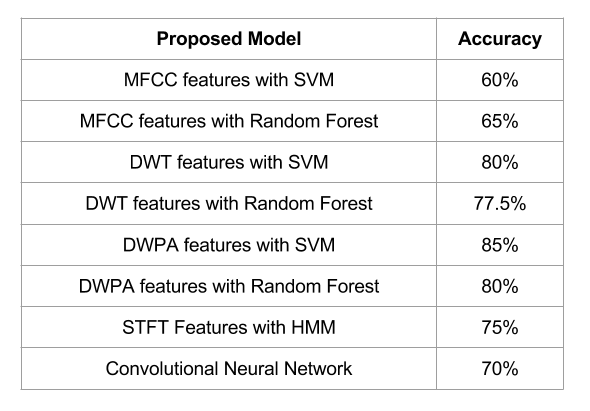
\includegraphics[scale=0.7]{./images/results.png}
\caption{Classification Results}
\end{figure}

\section{Complexity of Models}
Complexity of models depends on both complexity of feature extraction technique and classification algorithm.
Calculation of Fourier Transform has $O(N^2)$ complexity  which has very high computational cost when we have a long signal of N points. So one faster algorithm is proposed for this transform which is known as the Fast Fourier Transform(FFT). FFT has $O(N\log_{2}N)$ cost for calculation from N point signal. STFT  uses FFT as a building block, so  STFT takes $O(f* N \log{N})$ time where f is the number of frames because on each frame FFT takes $O(N \log{N})$  time. MFCC features are also based on  STFT so it involves same complexity because conversion from Hertz scale to Mel-scale require less time almost linear. Peak Detection algorithm first uses STFT and then a linear time procedure to separate out k peaks from f frames. When we calculate wavelet transform it takes $O(N)$ time using Fast Wavelet Transform (FWT) algorithm.\\


Complexity of the SVM algorithm depends on its complexity of quadratic optimization algorithm which is in the order of  $O(N\_samples^2 * N\_features)$ for RBF kernel using SMO solver and $O(N\_sample * N\_features)$ for linear SVM. We got the best result using radial basis function which involves inversion of kernel matrix which has complexity of order $O(n^3)$. Random forest constructs trees, so its complexity is number of trees times $O(v*n \log{n})$ where v is the number of feature and n is number of samples.  In HMM model Forward-Backward algorithm, Viterbi algorithm and Baum-Welch algorithm  has complexity of $O(T * N^2)$ where T is the length of sequence and N is the number of states. This runtime complexity in HMM is achieved when we have used dynamic programming approach.
In CNN, each layer has different type of operations which involves a lot of computation power. Complexity of CNN is very high because we have to perform a large number of iterations for forward propagation and back-propagation to learn the parameters of the network (weights in hidden layers).


\section{Conclusion from  Classification Results}
If we closely observe the results then we will find that when we extract MFCC feature using the STFT then it gives less accuracy compared to when we used wavelet feature because STFT does not do resolution in both time and frequency domain together while in wavelet (DWT or DWPA), we get information localized in both domains. With these feature extraction techniques SVM always outperforms Random Forest because SVM can be trained better on our small dataset.


In speech we also need information from previous state to model next state because all future events are dependent on previous events. So HMM is a great model for pattern analysis over time-series. HMM is generative model which tries to capture all changes in speech over time and generates probability of any testing speech samples to be generated using internal hidden states. HMM will perform better when trained with more observation so that it will be able to generalize the dataset.  Currently Deep Learning algorithms are  state of the art because in that we need not to know fixed kernel . Models like CNN will learn best kernel via back-propagation. These kernels will directly provide us all feature representation from low level features to object level features. In our case its accuracy is less because Convolution Neural Network is deep network with many layers which needs large data set to be trained upon. So this model may perform better if we use more number of samples to train.






\newpage
\chapter{Conclusions} 
\section{Summary of Work done}
First of all I read about what experiments were performed to record speech samples. Then I did a literature survey on work done related to my project such as methods for feature extraction from audio and classification algorithms. I listed and studied comparatively all popular methods to extract features from audio. These algorithms were very useful for this project (e.g. the Fourier transform, Gabor transform, wavelet transform, kernel methods using convolution for feature extraction). Then I analyzed spectrogram and scaleogram of all samples to find patterns among samples of the same class.\\
 For a classification task I pick Support Vector Machine because it can be trained easily to get tuned parameters even on small dataset and Random Forest because it is less prone to over-fit when number of features is very high in comparison to the number of samples. I pick Hidden Markov Model because it is used to model events which occur in time-series. Several variations of Hidden Markov Model have been proposed for time-series data and audio. At the end, I pick Convolution Neural Network because it automatically learns feature by convolution of kernels where these kernels are not fixed. These are estimated by several iterations of back-propagation algorithm in CNN which has many layers. 


\section{Contributions Made}
During literature survey I found there has been no published research work which tries to classify autistic and typical children using any machine learning technique. So I took decisions about which all signal processing methods are to be used for feature extraction and machine learning classification algorithms. We need a model which could identify characteristics of Autism Spectrum Disorder and predict whether a child is suffering from Autism Spectrum Disorder or not. To get such model I experimented with  different combination of feature extraction techniques and classification algorithms. With current dataset, feature extracted with the help of wavelet transforms (DWT and DWPA) and classified with Support Vector Machine outperforms other models. It will be very interesting to see which model will perform better with larger dataset.

\section{Future Work}
The future work in this project can be summarized as follows:
\begin{enumerate}
\item Collect more data set using cloud based android application which has launched at URL www.diseaseprediction.url.ph
\item Try to find some new set of articulatory features for classification by experimenting with different combination of feature extraction techniques.

\item Implement Convolutional Deep Belief Network with unsupervised classification to automatically cluster autistic and typical children.
\item Implement sequential deep learning approach for classification such as Recurrent Neural Networks. Emerging state of art for classification in this field is RNN-HMM model which is a combination of Recurrent Neural Network with Hidden Markov Model.
\end{enumerate}






\newpage



%\lhead{\emph{Bibliography}} % Change the page header to say "Bibliography"

\bibliographystyle{plain} % Use the "unsrtnat" BibTeX style for formatting the Bibliography

\bibliography{harshit} % The references (bibliography) information are stored in the file named "Bibliography.bib"




\newpage

\begin{center}
\textbf{ABOUT THE AUTHOR}\\[.5cm]
 \end{center}



\begin{minipage}[t]{0.65\linewidth} % [2]
\vspace{0pt} % [3]
The author is a student of M.Tech (Computer Technology) under the Electrical Engineering Department at Indian Institute of Technology Delhi at the time of this writing. He completed his B.Tech with honors in Computer Science of Engineering from Kamla Nehru Institute of Technology Sultanpur Uttar Pradesh Technical University. The author is interested to work in the areas of Machine Learning and Deep Learning. He is going to join McAfee (Intel Security) as a Sr. Software Engineer.
\end{minipage}
\hspace{0.5cm}
\begin{minipage}[t]{0.25\linewidth}
\vspace{0pt} % [3]
  \centering
  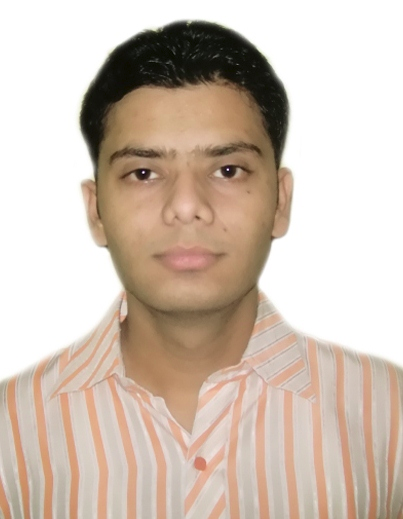
\includegraphics[width=\textwidth]{./images/myphoto.png}
\end{minipage}



\end{document}
